%%%%%%%%%%%%%%%%%%%%%%%%%%%%%%%%%%%%%%%%%%%%%%%%%%%%%%%
% A template for Wiley article submissions developed by 
% Overleaf for the Overleaf-Wiley pilot which ran 
% during 2017 and 2018.
% 
% This template is no longer supported, but is provided
% for historical reference. Last updated January 2019.
%
% Please note that whilst this template provides a 
% preview of the typeset manuscript for submission, it 
% will not necessarily be the final publication layout.
%
% Document class options:
% =======================
% blind: Anonymise all author, affiliation, correspondence
%        and funding information.
%
% lineno: Adds line numbers.
%
% serif: Sets the body font to be serif. 
%
% twocolumn: Sets the body text in two-column layout. 
% 
% num-refs: Uses numerical citation and references style 
%           (Vancouver-authoryear).
%
% alpha-refs: Uses author-year citation and references style
%             (rss).
%
% Using other bibliography styles:
% =======================
%
% To specify a different bibiography style
%
% 1) Do not use either num-refs or alpha-refs in documentclass.
% 2) Load natbib package with the options set as needed.
% 3) Use the \bibliographystyle command to specify the style
% 
% Included NJD styles are: 
%   WileyNJD-ACS
%   WileyNJD-AMA
%   WileyNJD-AMS
%   WileyNJD-APA
%   WileyNJD-Harvard
%   WileyNJD-VANCOUVER
%
% or you may upload an alternative .bst file 
% (if requested by the journal).
%
% Examples:
% =======================
%% Example: Using numerical, sort-by-authors citations.
\documentclass[num-refs,twocolumn]{wiley-article}

%% Example: Using author-year citations and anonymising submission
% \documentclass[blind,alpha-refs]{wiley-article}

%% Example: Using unsrtnat for numerical, in-sequence citations
% \documentclass{wiley-article}
% \usepackage[numbers]{natbib}
% \bibliographystyle{unsrtnat}

%% Example: Using WileyNJD-AMA reference style and superscript
%%          citations, two-column and serif fonts for AIChE
% \documentclass[serif,twocolumn,lineno]{wiley-article}
% \usepackage[super]{natbib}
% \bibliographystyle{WileyNJD-AMA}
% \makeatletter

% \makeatother

\usepackage{graphicx}
\usepackage{eso-pic}

% Ajout du logo en haut à droite de la première page
\AddToShipoutPictureBG*{
       \AtPageUpperLeft{%
              \put(\LenToUnit{\paperwidth-4cm},\LenToUnit{-2.6cm}){% Ajustez les coordonnées selon vos besoins
                     
\includegraphics[width=3cm]{Figures/logo-UT.png} % Remplacez 'example-image' par le chemin de votre logo
              }%
       }%
}
\AddToShipoutPictureBG*{
       \AtPageUpperLeft{%
              \put(\LenToUnit{\paperwidth-7cm},\LenToUnit{-2.8cm}){% Ajustez les coordonnées selon vos besoins
                     
\includegraphics[width=3cm]{Figures/Logo-CRBE.png} % Remplacez 'example-image' par le chemin de votre logo
              }%
       }%
}

\usepackage{siunitx}

% Update article type if known
\papertype{Résultats d'analyses}
\paperfield{Stage M1 Biodiversité Écologie Évolution}

\title{Composition et assemblage des communautés fongiques chez les plantes épiphytes vasculaires tropicales}

\author[1\authfn{1}]{Mathys Dussel--D'hervé}



\affil[1]{Faculté de Sciences et Ingénieurie - Université de Toulouse III - Paul Sabatier, 118 route de Narbonne, 31062 Toulouse Cedex 9, France}

\corraddress{Céline Leroy, Ecologie des Forêts de Guyane (UMR CNRS 8172), Campus Agronomique, 97379 Kourou Cedex, France}
\corremail{celine.leroy@utoulouse.fr}



\runningauthor{Mathys Dussel--D'hervé}
\begin{document}

\begin{frontmatter}
\maketitle

\begin{abstract}
Tropical forests harbor exceptional plant and microbial biodiversity that plays a critical role in ecosystem functioning and biogeochemical cycles. Among this diversity, vascular epiphytes are essential components of the tropical canopy, yet the composition and assembly of their associated fungal communities remain poorly understood. This study investigates the structure of fungal assemblages across different taxonomic groups of epiphytes, specifically comparing roots and leaves, as well as surface (episphere) versus internal tissues (endosphere). Utilizing samples collected in Peru and Colombia under the 'Life on Trees' program, fungal communities were characterized via high-throughput metabarcoding of the ITS region using Illumina MiSeq sequencing. Following bioinformatic processing, alpha and beta diversity will be analyzed using biodiversity indices, ordination methods (NMDS, PCoA), and multivariate statistical tests (PERMANOVA). This research aims to determine how host taxonomy and functional strategies for water and nutrient acquisition shape distinct fungal niches, providing a better understanding of plant-microorganism interactions within the tropical canopy.

\keywords{Vascular epiphytes, Tropical canopy, Fungal communities, Metabarcoding, ITS, Microbial ecology, Plant-microbe interactions, Biogeochemical cycles}
\end{abstract}
\end{frontmatter}

\section{Introduction}

Les forêts tropicales abritent une biodiversité végétale et microbienne exceptionnelle dont les interactions complexes régissent les cycles biogéochimiques et le maintien des fonctions écosystémiques. Au sein de la canopée, les plantes épiphytes vasculaires constituent une composante structurelle majeure, jouant un rôle déterminant dans la rétention d’eau et le recyclage des nutriments. Bien que leur importance écologique soit reconnue, les communautés microbiennes qui leur sont associées, et plus particulièrement le mycobiote, demeurent largement méconnues par rapport aux espèces ligneuses terrestres. Comprendre la composition et les mécanismes d’assemblage de ces communautés fongiques représente donc un enjeu de premier plan pour appréhender les symbioses en canopée et leur influence sur le fonctionnement des forêts tropicales.

La structuration de ces communautés fongiques pourrait être dictée par plusieurs filtres écologiques complémentaires. D'une part, la taxonomie de l'hôte pourrait exercer un contrôle sur les cortèges fongiques, reflétant une certaine spécificité entre la plante et ses partenaires microbiens. D'autre part, l'hétérogénéité des niches au sein d'un même individu, notamment entre les feuilles et les racines, suggère que les stratégies fonctionnelles d'acquisition des ressources influencent fortement la diversité microbienne. Enfin, le compartimentage entre la surface des organes (épisphère) et l'intérieur des tissus (endosphère) constitue une barrière environnementale et physiologique susceptible de sélectionner des taxons aux traits de vie distincts.

Pour tester ces hypothèses, cette étude s'appuie sur un échantillonnage conséquent réalisé au Pérou et en Colombie dans le cadre du programme « Life on Trees ». L’utilisation du métabarcoding haut débit ciblant la région ITS a permis de caractériser avec précision la diversité fongique associée à différentes espèces d'épiphytes. Les analyses statistiques, incluant des méthodes d'ordination NMDS et des tests de PERMANOVA, visent à quantifier l'influence respective du projet d'étude, de l'organe, de la position tissulaire et de la famille botanique de l'hôte sur l'assemblage des communautés. En complément, l'intégration de données microclimatiques permet d'explorer l'impact de gradients de température et d'humidité sur la richesse et la diversité fongique au sein de l'architecture complexe des arbres hôtes.

\section{Matériels et méthodes}

\paragraph{Échantillonnage et préparation des données}

L'étude a été conduite à partir d'échantillons de plantes épiphytes vasculaires collectés au Pérou et en Colombie dans le cadre du programme de recherche international « Life on Trees » (LOT). Afin de garantir la robustesse des analyses comparatives, le jeu de données initial a fait l'objet d'un filtrage rigoureux consistant à exclure les familles botaniques sous-représentées, telles que les Moraceae et les Fabaceae. Les séquences de la région ITS (Internal Transcribed Spacer) ont été obtenues par séquençage à haut débit sur plateforme Illumina MiSeq. Le traitement bioinformatique a permis de générer une table d'Unités Taxonomiques Opérationnelles (OTU) nettoyée, laquelle a été intégrée dans un objet de classe phyloseq sous l'environnement R. Pour les analyses de diversité bêta, une transformation de Hellinger a été appliquée aux abondances brutes afin de minimiser l'influence des taxons rares et de normaliser les écarts de profondeur de séquençage entre les échantillons.

\paragraph{Analyses de la diversité alpha et partage des taxons}

La diversité alpha a été caractérisée par deux indices complémentaires : la richesse spécifique observée ($q=0$) et l'exponentielle de l'indice de Shannon ($q=1$), cette dernière permettant une meilleure prise en compte de l'équitabilité des communautés. Les différences de diversité entre les groupes (organes, positions, projets) ont été évaluées par des tests non paramétriques de Kruskal-Wallis, suivis de tests de Wilcoxon par paires avec correction de Benjamini-Hochberg pour les comparaisons multiples. La distribution et le partage des OTU entre les différents compartiments (racines, jeunes feuilles, vieilles feuilles) ont été visualisés à l'aide de diagrammes de Venn, de graphiques UpSetR et de diagrammes de Chord. Ces approches ont permis d'identifier le "core microbiota" au niveau de la famille ainsi que les taxons partagés ou spécifiques à chaque niche écologique

\paragraph{Structure des communautés et analyses statistiques multidimensionnelles}

La structure globale des communautés fongiques a été explorée par des méthodes d'ordination en positionnement multidimensionnel non métrique (NMDS) basées sur des distances de Bray-Curtis. L'influence des facteurs structurants (projet, organe, position et taxonomie de l'hôte) sur la composition fongique a été quantifiée par des analyses de variance moléculaire de type PERMANOVA (fonction adonis2, 99 permutations). Parallèlement, l'homogénéité de la dispersion des communautés a été vérifiée par des tests de permutation sur les variances (betadisper). Pour identifier les taxons présentant des abondances différentielles significatives entre les organes, l'outil statistique ANCOM-BC2 (Analysis of Compositions of Microbiomes with Bias Correction) a été utilisé, appliquant une correction de Holm pour les valeurs de p.

\paragraph{Caractérisation fonctionnelle et niche écologique}

L'annotation fonctionnelle des OTU a été réalisée par l'interpellation de la base de données FungalTraits, permettant d'assigner des modes de vie (saprotrophes, pathogènes, endophytes) aux taxons identifiés au niveau de l'espèce. L'influence des facteurs environnementaux et taxonomiques sur ces traits fonctionnels a été testée par une analyse canonique des corrélations (ACC), dont la significativité des termes a été évaluée par des tests de permutation. Enfin, la largeur de niche fongique par organe a été estimée via l'indice de Levins normalisé (compris entre 0 pour les spécialistes et 1 pour les généralistes), calculé sur les abondances fusionnées par type d'organe.

\paragraph{Modélisation du microclimat et de la richesse spécifique}

L'impact des variables microclimatiques sur la diversité fongique a été analysé pour le site LOT1 en utilisant les mesures de température et d'humidité enregistrées sur différentes zones de l'arbre (base, tronc, cœur, périphérie de la canopée). Les relations entre ces variables et la richesse spécifique (Observed) ou la diversité (ExpShannon) ont été modélisées à l'aide de modèles linéaires généralisés à distribution binomiale négative (GLM-NB), permettant de gérer la surdispersion des données de comptage. La validité de ces modèles a été contrôlée par l'analyse des résidus simulés avec le package DHARMa, incluant des tests d'uniformité, de dispersion et de zéro-inflation.

\section{Résultats}

\paragraph{Diversité alpha et partage des communautés}

L'analyse de la diversité alpha révèle des contrastes marqués selon les compartiments de la plante épiphyte. La richesse spécifique observée (q=0) et la diversité de Shannon (q=1) montrent des tendances significatives entre les racines et les feuilles, ainsi qu'entre l'épisphère et l'endosphère (Tests de Kruskal-Wallis, p<0.05). Les racines présentent généralement une richesse en OTU plus élevée que les tissus foliaires. L'analyse des diagrammes de Venn et UpSetR met en évidence un faible partage de taxons entre les racines et les feuilles, suggérant une forte spécialisation des niches. Bien que certains taxons soient ubiquistes, une large fraction des OTU est strictement inféodée à un type d'organe ou à une position (endosphère vs épisphère), soulignant l'importance du micro-habitat dans la sélection des communautés fongiques.

\begin{figure*}[t]
    \centering

    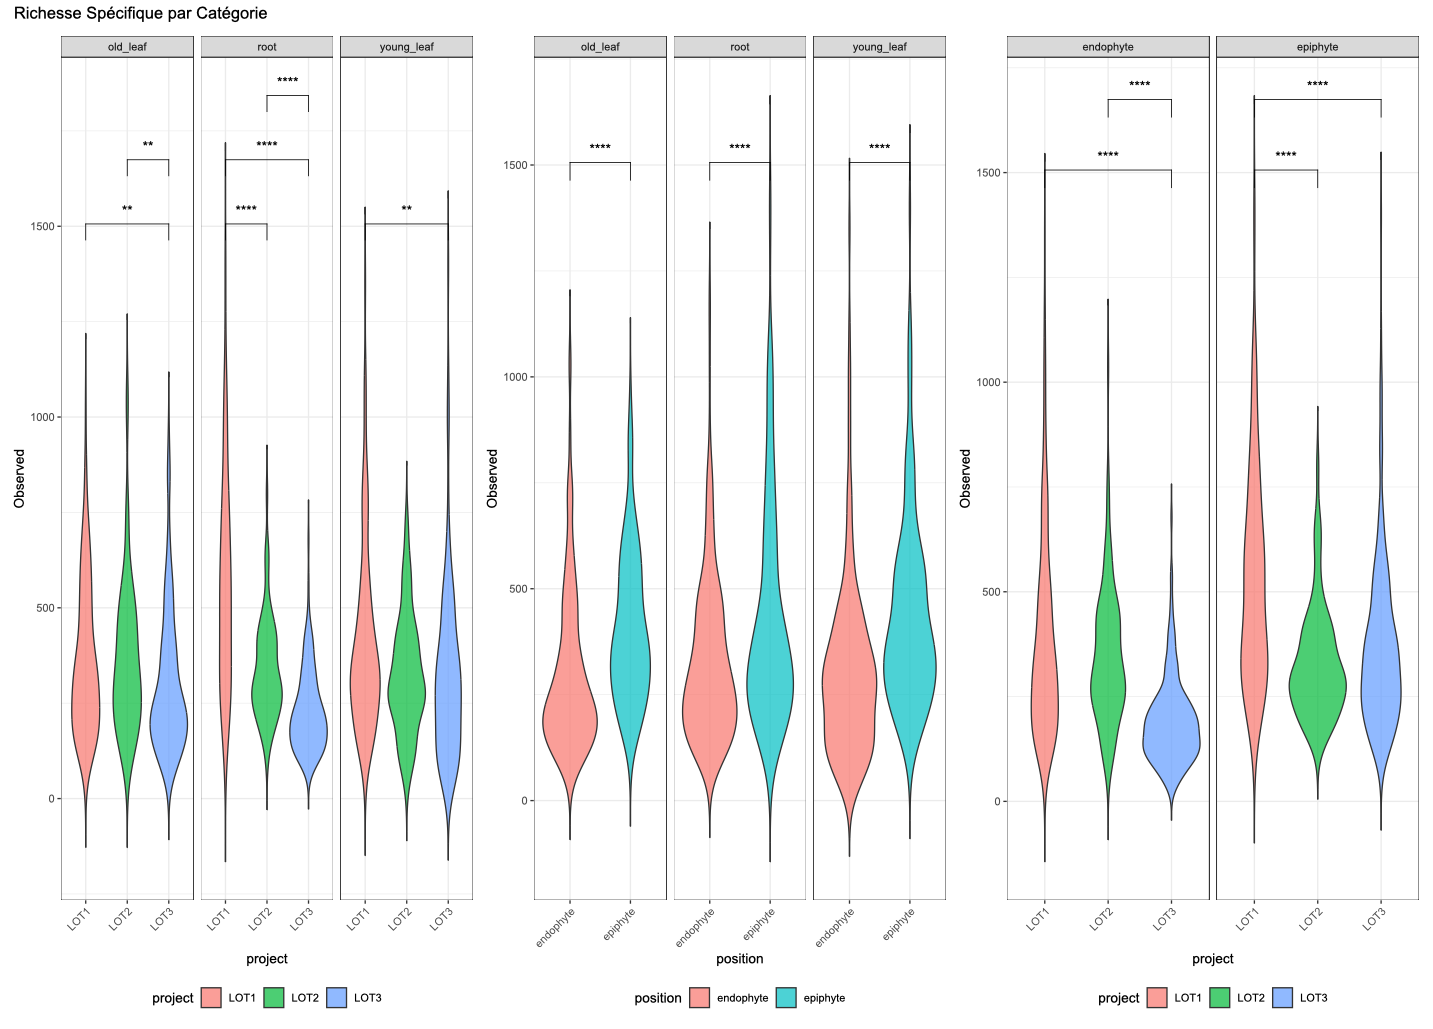
\includegraphics[width=0.4\linewidth]{Figures/plot-30.png} 
       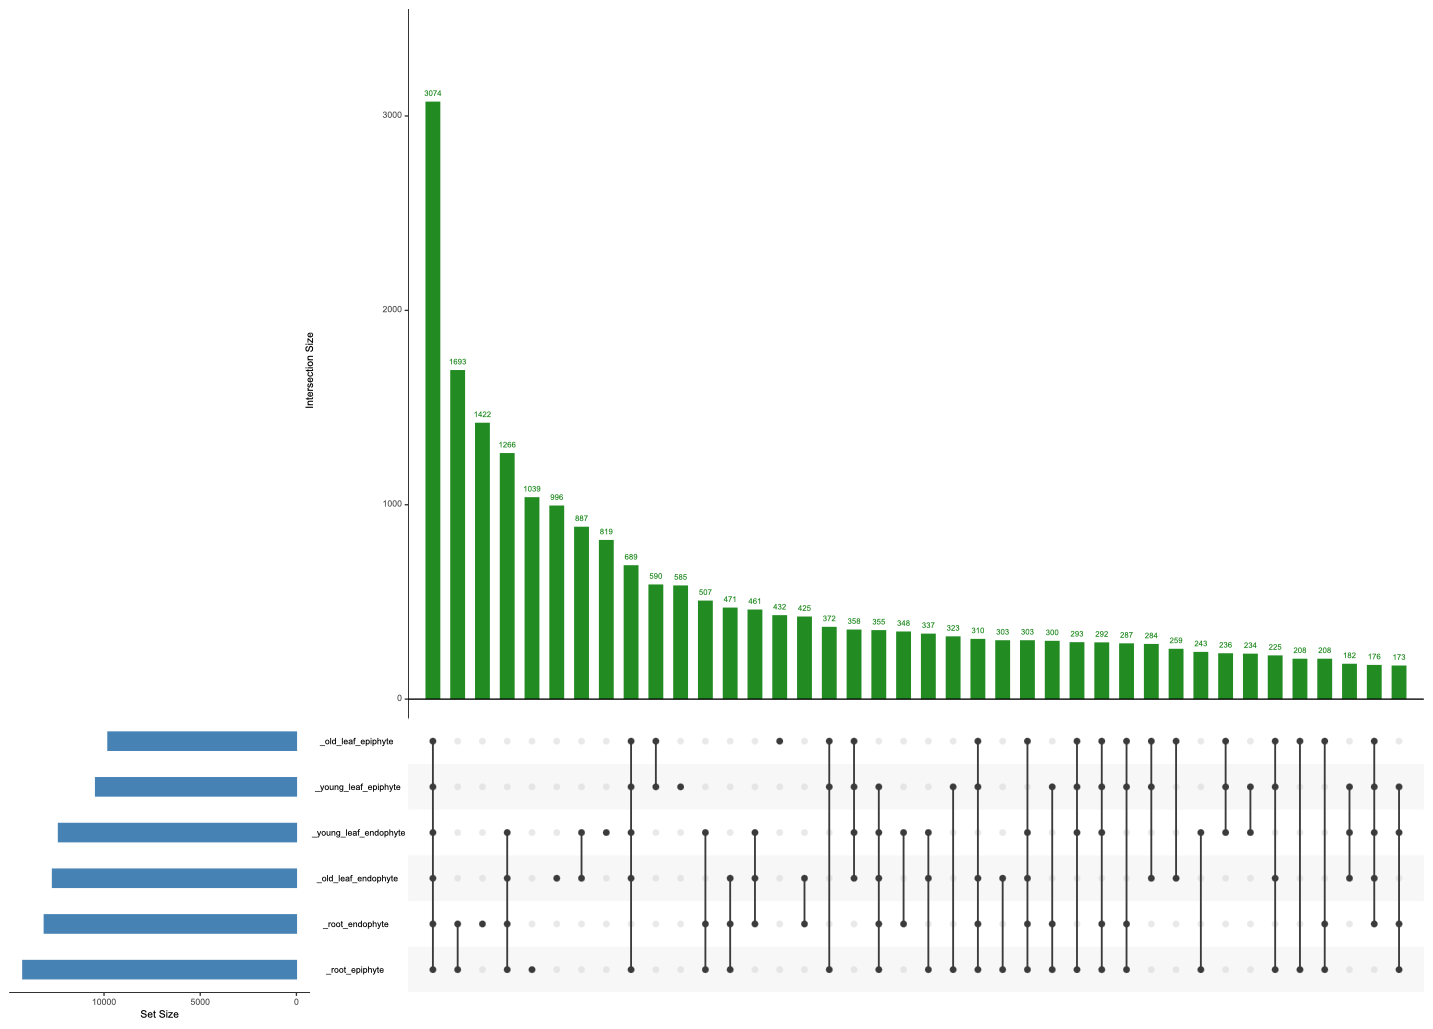
\includegraphics[width=0.5\linewidth]{Figures/plot-36.png} 
    \caption{Diversité alpha des communautés fongiques. (gauche) Richesse spécifique observée et indice de Shannon selon l'organe et la position. (droite) Diagramme UpSet illustrant les taxons exclusifs et partagés entre les niches.}
    \label{fig:alpha_results}
\end{figure*}

\paragraph{Structuration des communautés (Diversité bêta)}

L'ordination par positionnement multidimensionnel non métrique (NMDS) montre une structuration nette des communautés fongiques. À l'échelle globale, le facteur "Projet" (site d'étude) explique une part significative de la variance ($R^2=0.108, p<0.01$). Toutefois, des analyses plus fines révèlent que l'organe (racine vs feuille) et la position (endophyte vs épiphyte) sont des déterminants majeurs de la composition du mycobiote. L'ordination globale (Stress = 0.13, k=3) affiche une séparation claire entre les échantillons racinaires et foliaires. Les tests de PERMANOVA confirment que la famille botanique de l'hôte exerce également un contrôle significatif sur l'assemblage fongique, bien que son effet soit parfois secondaire par rapport à la différenciation des organes.

\paragraph{Compositions taxonomiques et niches fonctionnelles}

Les diagrammes de Chord et les analyses d'abondances relatives indiquent une dominance de certains groupes taxonomiques selon les niches. Les communautés sont largement dominées par les Ascomycota et les Basidiomycota, mais les proportions de classes varient : les racines hébergent une diversité fonctionnelle distincte de celle des feuilles. L'indice de Levins calculé montre que les communautés fongiques foliaires ont tendance à présenter des niches plus étroites (spécialisation plus forte) par rapport aux communautés racinaires. L'analyse fonctionnelle via FungalTraits révèle une prédominance de taxons saprotrophes dans l'épisphère, tandis que les symbiotes et endophytes potentiels sont plus représentés dans l'endosphère.


\paragraph{Influence des variables microclimatiques}

Les modèles linéaires généralisés (GLM-NB) appliqués aux données du site LOT1 démontrent une influence significative des facteurs environnementaux sur la richesse fongique. L'humidité relative moyenne et la température interagissent pour structurer la diversité. Les tests de diagnostic (DHARMa) valident la robustesse des modèles, ne montrant ni surdispersion (p=0.835) ni inflation de zéros (p=1). Une humidité élevée couplée à des températures stables dans les zones protégées de l'arbre (cœur de la canopée, base) favorise une richesse spécifique plus élevée par rapport à la périphérie de la canopée, soumise à des stress hydriques plus importants.

\section{Discussion}

\bibliography{bibliographie.bib}

\listoffigures
\listoftables

\appendix
\section{Annexes}

\end{document}